הדוגמה הבאה ממחישה את הטענה על מרחק הצמתים מ-$s$. 
מסלול השיפור בכל איטרציה מסומן בכתום, הניחו כי כל הקיבולים שווים.
שימו לב למרחק הצמתים 4 ו-7 מ-$s$.
\begin{center}
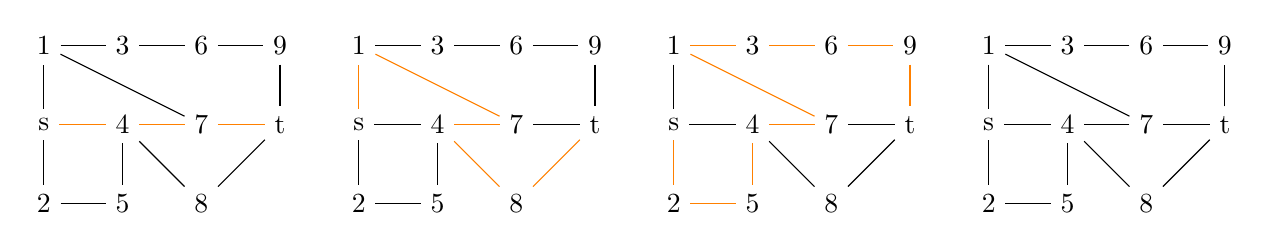
\begin{tikzpicture}[]

%%%% 1
%%%%
\begin{scope}
\node(s) at(0,0) {s};
\foreach[count=\i] \x \y in{
0/1,0/-1,1/1,1/0,1/-1,2/1,2/0,2/-1,3/1%
}{
\node(\i) at(\x,\y) {\i};
}
\node(t) at(3,0) {t};

\foreach \u \v in{
s/1,s/2,1/3,1/7,2/5,3/6,4/8,5/4,6/9,8/t,9/t%
}{
\draw[] (\u) -- (\v);
}

\foreach \u \v in{
s/4,4/7,7/t%
}{
\draw[orange] (\u) -- (\v);
}

\end{scope}

%%%% 2
%%%%
\begin{scope}[xshift=4cm]
\node(s) at(0,0) {s};
\foreach[count=\i] \x \y in{
0/1,0/-1,1/1,1/0,1/-1,2/1,2/0,2/-1,3/1%
}{
\node(\i) at(\x,\y) {\i};
}
\node(t) at(3,0) {t};

\foreach \u \v in{
s/2,4/s,1/3,2/5,3/6,5/4,6/9,t/7,9/t%
}{
\draw[] (\u) -- (\v);
}

\foreach \u \v in{
s/1,1/7,7/4,4/8,8/t%
}{
\draw[orange] (\u) -- (\v);
}

\end{scope}

%%%% 3
%%%%
\begin{scope}[xshift=8cm]
\node(s) at(0,0) {s};
\foreach[count=\i] \x \y in{
0/1,0/-1,1/1,1/0,1/-1,2/1,2/0,2/-1,3/1%
}{
\node(\i) at(\x,\y) {\i};
}
\node(t) at(3,0) {t};

\foreach \u \v in{
1/s,4/s,8/4,t/7,8/t%
}{
\draw[] (\u) -- (\v);
}
\foreach \u \v in{
s/2,2/5,5/4,4/7,7/1,1/3,3/6,6/9,9/t%
}{
\draw[orange] (\u) -- (\v);
}
\end{scope}

%%%% 4
%%%%
\begin{scope}[xshift=12cm]
\node(s) at(0,0) {s};
\foreach[count=\i] \x \y in{
0/1,0/-1,1/1,1/0,1/-1,2/1,2/0,2/-1,3/1%
}{
\node(\i) at(\x,\y) {\i};
}
\node(t) at(3,0) {t};

\foreach \u \v in{
1/s,4/s,8/4,t/7,8/t%
,2/s,5/2,4/5,7/4,1/7,3/1,6/3,9/6,t/9%
}{
\draw[] (\u) -- (\v);
}
\end{scope}

\end{tikzpicture}
\end{center}
